\begin{figure}[!htbp]
\centering
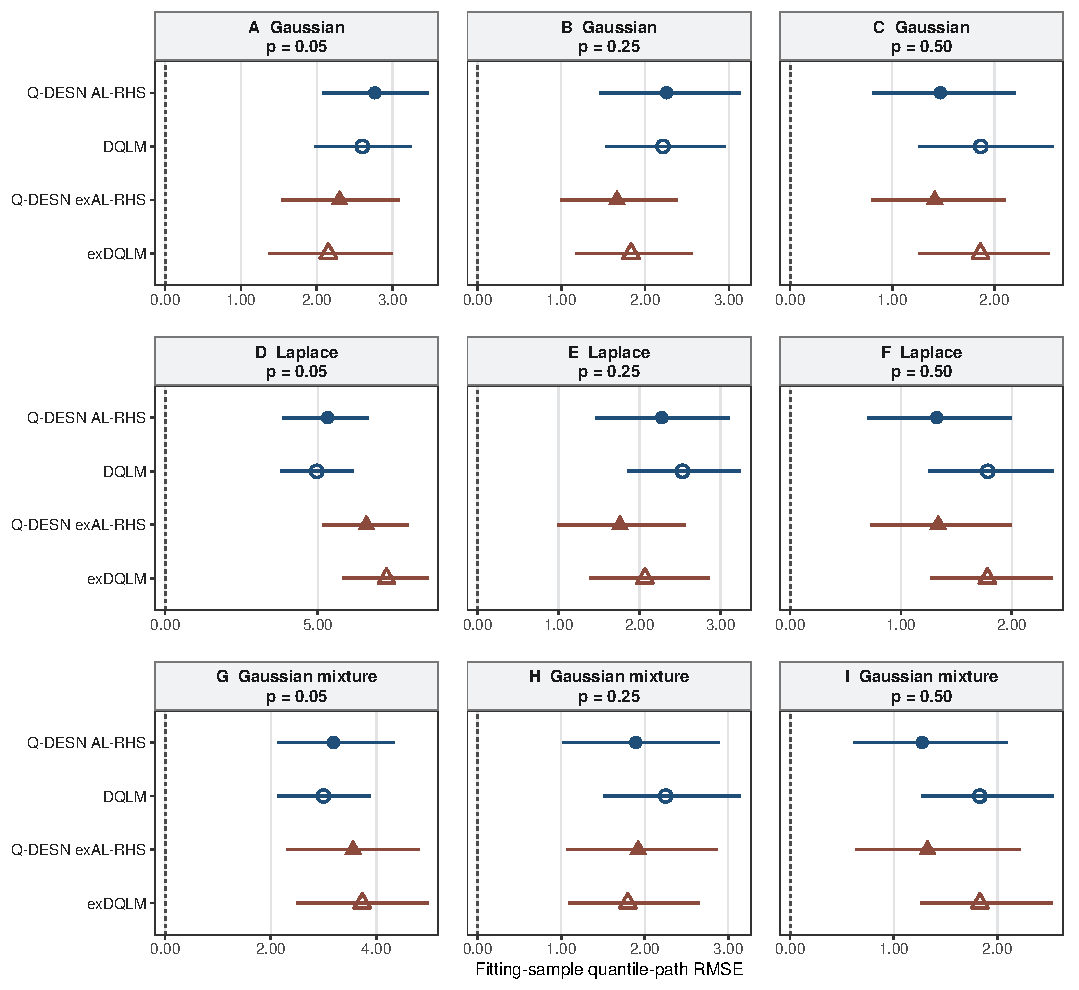
\includegraphics[width=0.98\textwidth]{figures/ch04-qdesn/independent_simulation/qdesn_validation_500obs_v14_mcmc_fit_rmse_intervals.pdf}
\caption{MCMC fitting-sample recovery in the single-quantile simulation.
Points are posterior means of quantile-path root mean squared error (RMSE) and
horizontal segments are equal-tailed 95\% posterior intervals; lower values
are better. Navy circles identify the \(\AL\) models and muted-brick triangles
the \(\exAL\) models; filled symbols denote Q--DESN and open symbols the
corresponding dynamic quantile linear model. Panels A--I identify the
data-generating family and probability level and use separate horizontal
scales. The dashed line marks exact recovery of the known conditional quantile
path. Intervals condition on the simulated series and case-specific selected
specification.}
\figalt{Nine panels compare posterior fitting-sample quantile-path RMSE means
and 95 percent intervals for four models across three innovation families and
three probability levels. Lower values are better.}
\label{qdesn:fig:simulation-500obs-mcmc-fit-rmse-intervals}
\end{figure}
